% The Warsaw circle: the topologist's sine curve, its limiting segment, and an
% elliptical arc closing the two ends up.
% Source: book/tex/topology/cover-project.tex (§ The lifting criterion).
\documentclass[border=2mm]{standalone}
\usepackage{tikz}
\begin{document}
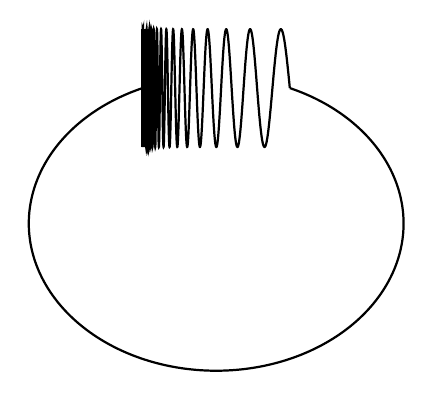
\begin{tikzpicture}[scale=3.4]
  % limiting segment {0} x [-h, h]
  \draw[line width=1.1pt] (0,-0.22) -- (0,0.22);
  % y = h sin(k log(w/x)) for x in (0, w], sampled densely towards x = 0
  \draw[line width=0.8pt,domain=0:1,samples=3000,smooth,variable=\t]
    plot ({0.55*exp(-8*\t)}, {0.22*sin(deg(25*8*\t))});
  % arc from (w, 0) round the outside back to the segment
  \draw[line width=0.8pt,domain=66.86:-246.86,samples=400,smooth,variable=\a]
    plot ({0.275 + 0.7*cos(\a)}, {-0.5057 + 0.55*sin(\a)});
\end{tikzpicture}
\end{document}
